\chapter{Hardware}
%http://samurai1967.dyndns.org/avr-net-io.html
%http://www.fhemwiki.de/wiki/AVR-NET-IO
%http://www.mikrocontroller.net/articles/AVR_Net-IO_Bausatz_von_Pollin
\section{AVR Net-IO-Board}
\begin{figure}[h]
\centering
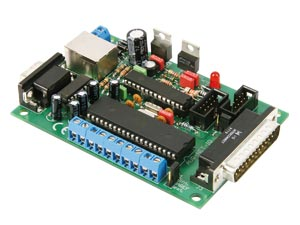
\includegraphics[width=10cm]{content/pictures/avr-net-io.jpg}
\caption{AVR-NET-IO - Pollin GmbH}
%http://www.pollin.de/shop/dt/MTQ5OTgxOTk-/Bausaetze_Module/Bausaetze/Bausatz_AVR_NET_IO.html
\label{fig:B3}
\end{figure}

\subsection{Technische Daten}
\begin{itemize}
  \item Betriebsspannung 9V
  \item Stromaufnahme ca. 190 mA
  \item 8 Digitale Ausgänge, 4 Digitale Eingänge
  \item 4 Analoge Eingänge
  \item ATmega32 Mikrocontroller
  \item integrierte ISP-Schnittstelle
\end{itemize}

\section{Mikrocontroller}
\subsection{ATmega32}

\subsection{ATmega644P}

\subsection{ATmega1284P}

\subsection{ENC28J60}

\section{Fuse Bits}
\label{chap:Fuse}

Die Fuse-Bits sind die Grundlegenden Einstellungen, mit denen ein
Mikrocontroller arbeitet. Sie müssen geändert werden, wenn ein anderer Taktgeber
gewünscht ist oder Schnittstellen de- oder aktiviert werden sollen.

\begin{myframe}
\textbf{Allgemeiner Hinweis:} Dieser Artikel kann die Recherche im Datenblatt
nicht ersetzen, besonders bei abweichendem Mikrocontroller sind die Fuse-Bits
oft anders gewählt. Mit dem Atmel Studio kann es vorkommen, dass man sich vom
Mikrocontroller aussperrt. Ein zurücksetzen der Fuse-Bits kann mit AVRDUDE
in diesem Fall versucht werden. Beschrieben wird dieser Vorgang im
Benutzerhandbuch \ref{Chapt:Einrichten}
\end{myframe}

In Tabelle ref{fuses-names} werden die einzelnen Fuse-Bits zusammen mit ihrer
Bedeutung und dem entsprechendem Byte aufgelistet. Der Schlussendliche Fuse Wert
setzt sich aus zwei Byte zusammen, wobei eine 1 eine deaktivierte Eigenschaft und
eine 0 aktiviert Eigenschaft bedeutet. Kleinere Mikrocontroller besitzen nur ein
High (H) und ein Low (L) Register, größere Mikrocontroller besitzen zusetzlich
noch ein Extended (E) Register.

\begin{table} [H]
\begin{tabular}{|l|l|l|} \hline
Fuse Name & Bedeutung & Bytes\\ \hline
BODLEVEL & Brown-out Detector trigger level & E-Fuse 0\&1\\ \hline
OCDEN & Aktiviert On-Chip Debuging & H-Fuse 7\\ \hline
JTAGEN & Aktiviert das \ac{JTAG} Interface & H-Fuse 6\\ \hline
SPIEN & Aktiviert das \ac{ISP} Interface & H-Fuse 5\\ \hline
WDTON & \ac{WDT} immer an & H-Fuse 4\\ \hline
EESAVE & Schützt den \acs{EEPROM} wärend des Lösch-Zyklus & H-Fuse 3\\ \hline
BOOTSZ & Boot Flash Sektor Größe & H-Fuse 1\&2\\ \hline
BOOTRST & Boot Reset Vektor & H-Fuse 0\\ \hline
CKDIV8 & Teilt den Takt der Uhr intern durch 8 & L-Fuse 8\\ \hline
CKOUT & Ausgabe des Takts der Uhr auf Port B1 & L-Fuse 7\\ \hline
SUT\_CKSEL & Wahl der Takt-Quelle & L-Fuse 0-6\\ \hline
\end{tabular}
\caption{Die Bedeutung der einzelnen Fuse-Bits (ATMega-664P)}
\label{fuses-names}
\end{table}

Wir benötigen für unseren ATMega-664P SPIEN, EESAVE und BOOTRST aktiviert im
High Register. Im Low Register muss alles deaktiviert werden, damit die Externe
Quarz-Kristall verwendet wird. Da das Brown-out Detector trigger level nicht
verwendet wird, kann in den Extended Register es ebenfalls alles deaktiviert
werden. Daraus resultiert die Bit Kombination in Tabelle \ref{fuses-result}.

\begin{table}[H]
\centering
\begin{tabular}{|l|l|l|} \hline
Fues Register & Binär & Hex\\ \hline
Extended-Fuse & 1111 1111 & FF\\ \hline
High-Fuse & 1101 0110 & D6\\ \hline
Low-Fuse & 1111 1111 & FF\\ \hline
\end{tabular}
\caption{Fuse Einstellungen (ATMega-664P)}
\label{fuses-result}
\end{table}

Im Atmel Studio können die Fuse Einstellungen ganz einfach im Device Programming
vorgenommen werden (Kapitel \ref{Chap:atmelStudio.Programming}). In Abbildung
\ref{fuses-graf} können sind die festgelegten Einstellungen eingetragen.

\begin{figure}[h]
\centering
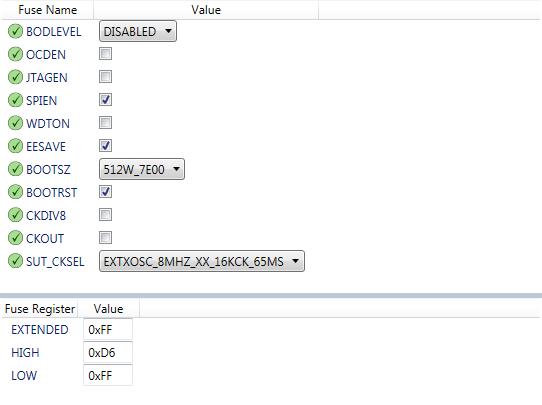
\includegraphics[width=13cm]{content/pictures/Fusebits/fusebits_atmelstudio.png}
\caption{Fuse-Bits im Atmel Studio (ATMega-664P)}
\label{fuses-graf}
\end{figure}

